%
% To make graphic on linux....(require ImageMagic installed)
%
% pdflatex thisfile.tex
% convert -density 300 thisfile.pdf -resize 640x480 thatfile.png 
%
% On Windows 10.... copy ImageMagic's convert.exe to your path 
% or rename it imgconvert.exe
% Get recent version of GhostScript
%
% pdflatex thisfile.tex
% convert -density 300 thisfile.pdf -resize 640x480 thatfile.png 
%
% Trouble? See this thread
%
% https://tex.stackexchange.com/questions/11866/compile-a-latex-document-into-a-png-image-thats-as-short-as-possible/11880#11880
%
\documentclass{standalone}
\usepackage{tikz}
\author{CC-BY-2016 James B. Wilson}
\date{\toay}
\begin{document}
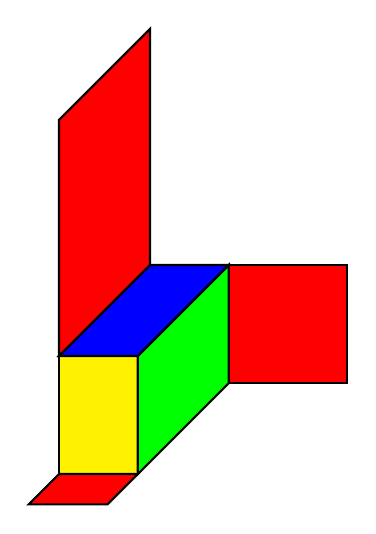
\begin{tikzpicture}[scale=0.25]
\pgfmathsetmacro{\cubex}{4}
\pgfmathsetmacro{\cubey}{6}
\pgfmathsetmacro{\cubez}{12}
\draw[black,thick,fill=yellow] (0,0,0) -- ++(-\cubex,0,0) -- ++(0,-\cubey,0) -- ++(\cubex,0,0) -- cycle;
\draw[black,thick,fill=green] (0,0,0) -- ++(0,0,-\cubez) -- ++(0,-\cubey,0) -- ++(0,0,\cubez) -- cycle;
\draw[black,thick,fill=blue] (0,0,0) -- ++(-\cubex,0,0) -- ++(0,0,-\cubez) -- ++(\cubex,0,0) -- cycle;
\draw[black, thick,fill=red] (0,-\cubey,0) -- ++(-\cubex,0,0) -- ++(0,0,\cubex) -- ++(\cubex,0,0) -- cycle;
\draw[black, thick,fill=red] (-\cubex,0,0) -- ++(0,0,-\cubez) -- ++(0,\cubez,0) -- ++(0,0,\cubez) -- cycle;
\draw[black, thick,fill=red] (0,0,-\cubez) -- ++(\cubey,0,0) -- ++(0,-\cubey,0) -- ++(-\cubey,0,0) -- cycle;
\end{tikzpicture}
\end{document}


